\documentclass[13pt]{beamer}
\usepackage{tikz}
\usepackage[french]{babel}
\usepackage{url}
\usepackage{caption}
\usepackage{xcolor}
\usepackage{listings}
\lstset{basicstyle=\ttfamily,
  showstringspaces=false,
  commentstyle=\color{red},
  keywordstyle=\color{blue}
}

\definecolor{blackRobotronik}{RGB}{19,19,19}

% setting some colors for the theme
\setbeamercolor{palette primary}{fg=blackRobotronik,bg=white}
\setbeamercolor{palette secondary}{fg=blackRobotronik,bg=white}
\setbeamercolor{structure}{fg=white,bg=blackRobotronik}
\setbeamercolor{title in head/foot}{fg=white,bg=blackRobotronik}
\setbeamercolor{date in head/foot}{fg=white,bg=blackRobotronik}

% definition of the footline template
\defbeamertemplate*{footline}{Robotronik}{%
  \leavevmode%
  \hbox{\begin{beamercolorbox}[wd=.5\paperwidth,ht=2.5ex,dp=1.125ex,leftskip=.3cm,rightskip=.3cm]{title in head/foot}%
    \makebox[2em][l]{{\usebeamerfont{title in head/foot}\textcolor{blackRobotronik}{\insertframenumber}}}%
    {\usebeamercolor{title in head/foot}\insertframenumber}
  \end{beamercolorbox}%
  \begin{beamercolorbox}[wd=.2\paperwidth,ht=2.5ex,dp=1.125ex,leftskip=.3cm,rightskip=.3cm]{date in head/foot}%
    \usebeamerfont{date in head/foot}\insertshorttitle%
  \end{beamercolorbox}%
  \begin{beamercolorbox}[wd=.3\paperwidth,ht=2.5ex,dp=1.125ex,leftskip=.3cm,rightskip=.3cm]{title in head/foot}%
  \insertshortdate
    %\includegraphics[width=.2\paperwidth,height=2.5ex,keepaspectratio]{gemalto}\hspace*{2em}%
  \end{beamercolorbox}}%
  \vskip0pt%
}

% definition of the title page template
\defbeamertemplate*{title page}{Robotronik}[1][]
{%
  \begin{tikzpicture}[remember picture,overlay]
  \filldraw[blackRobotronik]
    (current page.north west) --
    ([yshift=-2cm]current page.north west) --
    ([xshift=-2cm,yshift=-2cm]current page.north east) {[rounded corners=15pt]--
    ([xshift=-2cm,yshift=3cm]current page.south east)} --
    ([yshift=3cm]current page.south west) --
    (current page.south west) --
    (current page.south east) --
    (current page.north east) -- cycle
    ;
  \node[text=blackRobotronik,anchor=south west,font=\sffamily\LARGE,text width=.55\paperwidth] 
  at ([xshift=10pt,yshift=-1cm]current page.west)
  (title)
  {\raggedright\inserttitle};   
  \node[anchor=west]
  at (title.east)
  {
\includegraphics[height=2.25cm]{Images/logo.png}};
  \node[text=white,font=\large\sffamily,anchor=south west]
  at ([xshift=30pt,yshift=1cm]current page.south west)
  (date)
  {\insertdate};
  \node[text=white,font=\large\sffamily,anchor=south west]
  at ([yshift=5pt]date.north west)
  (author)
  {\insertauthor};
  \end{tikzpicture}%
}

% remove navigation symbols
\setbeamertemplate{navigation symbols}{}

\setbeamertemplate{itemize item}[circle]
\setbeamercolor{itemize item}{fg=blackRobotronik}
\setbeamertemplate{itemize subitem}[square]
\setbeamercolor{itemize subitem}{fg=blackRobotronik}
\setbeamertemplate{itemize subsubitem}[cicle]
\setbeamercolor{itemize subsubitem}{fg=blackRobotronik}

\newenvironment{slide}[1]{
  \begin{frame}[environment=slide]
    \frametitle{\textbf{\insertsection}  : #1}}
{\end{frame}}

\setbeamercolor{section in toc}{fg = blackRobotronik}
\setbeamercolor{section in toc shaded}{fg = blackRobotronik}
\setbeamertemplate{section in toc}[square]
\setbeamerfont{section number projected}{size=\large}
\setbeamercolor{section number projected}{bg=blackRobotronik,fg=white}

\setbeamercolor{caption name}{fg=blackRobotronik}
\setbeamertemplate{caption}[numbered]
\setbeamercolor{caption number}{fg=blackRobotronik}

\title{Linux, les bases}
\author{Nicolas Cubric}
\date{13/11/2019 - M001}

\begin{document}

\begin{frame}
\maketitle
\end{frame}

\begin{frame}
  \frametitle{\textbf{Sommaire}}
  \tableofcontents
\end{frame}

\section{Introduction}
\subsection{Linux c'est quoi ?}

\begin{slide}{Linux c'est quoi ?}
  \begin{center}
    
\includegraphics[scale=0.25]{Images/GNU_TUX.png}
    \captionof{figure}{Logo de GNU/Linux}
  \end{center}
\end{slide}

\begin{slide}{Linux c'est quoi ?}
  \begin{itemize}
    \item Un système d'exploitation
      \begin{itemize}
        \item crée en 1991 par Linus Torvalds.
        \item écrit en C et en assembleur
      \end{itemize}
    \item Utilisé de partout
    \begin{itemize}
      \item Ordinateurs personnel
      \item Téléphones portables/Tablettes
      \item Super-ordinateurs
    \end{itemize}
  \end{itemize}
\end{slide}

\subsection{Les distributions}

\begin{slide}{Les distributions}
  \begin{center}
    
\includegraphics[scale=0.5]{Images/distro_mosaic.png}
    \captionof{figure}{Logo de différentes distributions}
  \end{center}
\end{slide}

\section{L'arborescence}

\begin{slide}{}
  \begin{center}
    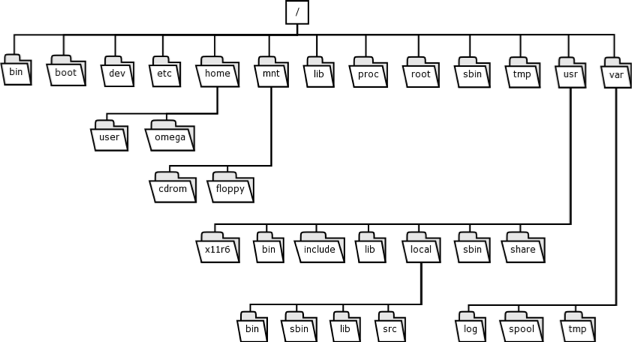
\includegraphics[scale=0.3]{Images/arborescence.png}
    \captionof{figure}{Arborescence dans Linux}
  \end{center}
\end{slide}

\begin{slide}{/}
  \begin{itemize}
  \item C'est le dossier à la racine.
  \item Son petit nom c'est root (comme racine en anglais)
  \item De ce dossier pars tout l'arborescence du systéme
  \item Nous allons voir les principals dossiers.
  \end{itemize}
\end{slide}

\begin{slide}{/home}
  \begin{itemize}
  \item C'est la maison !!!
  \item Ici on retrouve toutes les données des utilisateurs
  \item Chaques utilisateurs à son dossier attitré
  \end{itemize}
\end{slide}

\subsection{Retrouver son chemin}

\begin{slide}{Retrouver son chemin}
  Il existe deux types de chemins dans Linux :
  \begin{itemize}
    \item Les chemins \textit{absolus}
      \begin{itemize}
      \item On exprime le chemin en partant de la racine
      \item Par exemple le chemin pour mon home : /home/nikola
      \end{itemize}
    \item Les chemins \textit{relatifs}
      \begin{itemize}
      \item On exprime le chemin relatif au dossier courant.
      \item Par exemple le chemin pour mon home : \textasciitilde
      \end{itemize}
  \end{itemize}
\end{slide}

\begin{slide}{Chemin relatif ?}
  Comme préciser dans slide précédente, il est possible d'exprimer un chemin par
  rapport au dossier dans lequel on se situe.\\

  Si l'on affiche les fichier cacher on peut remarquer deux dossiers présents
  peu importe où l'on se situe dans l'arborescence :
  \begin{itemize}
  \item . qui est le dossier courant
  \item .. qui est le dossier parent
  \end{itemize}
\end{slide}

\section{Quelques commandes de bases}

\subsection{Le terminal}
\begin{slide}{Le terminal}
  \begin{itemize}
  \item Dans la majorité des interfaces graphique : ctr+alt+t
  \item Sinon aller chercher dans la liste des applications
  \end{itemize}
\end{slide}

\subsection{man}

\begin{slide}{man}
  \begin{itemize}
  \item man pour manual
  \item Utile quand on cherche des informations sur une commande
  \end{itemize}
  \begin{center}
    \large{Exemple d'utilisation :\\
      \textbf{À vos pcs !!!}}
  \end{center}
\end{slide}


\section{Conclusion}

\begin{frame}
  \frametitle{\textbf{Conclusion}}
  Merci de votre attenion.\\
  \vspace*{1cm}
  Les slides et sont disponibles sur le github de Robotronik : \url{github.com/robotronik/conferences}
\end{frame}


\end{document}